\documentclass[11pt]{article}
\usepackage[margin=0.85in]{geometry}
\usepackage{amsmath,amssymb,graphicx,booktabs,xcolor,float,enumitem,bm}
\usepackage[T1]{fontenc}
\usepackage{lmodern}
\usepackage{hyperref}
\hypersetup{colorlinks=true,linkcolor=blue!60!black,urlcolor=blue!60!black,citecolor=blue!60!black}
\graphicspath{{../v6/}}
\newcommand{\hmpc}{\,h\,\mathrm{Mpc}^{-1}}
\newcommand{\kmax}{k_{\max}}
\newcommand{\PNL}{P_{\rm NL}}
\newcommand{\Plin}{P_{\rm lin}}
\newcommand{\bTA}{b_{\rm TA}}
\newcommand{\dd}{\mathrm{d}}
\title{A halo model for intrinsic alignments with central-galaxy\\1-halo alignment: review}
\author{Yijie Zhu, with Claude}
\date{11 November 2026; addendum 17 November 2026}

\begin{document}
\maketitle

\section*{Summary}
\begin{itemize}[itemsep=3pt]
\item \textbf{Correction, 17 November 2026 (Sec.~\ref{sec:addendum}).} The
  central 1-halo amplitudes fitted to FLAMINGO below ($a_c = 13$ to 190) are 30
  to 400 times the physical size of that amplitude ($a_c \simeq 0.5$ for a
  central that copies the shape of its halo). They compensate for nonlinear
  power that the $\PNL \to I_1\Plin$ swap removes from the 2-halo term. With a
  share $\alpha \approx 0.4$ to 0.8 of that power restored and $a_c \le 1$ the
  fits are as good or better, and FLAMINGO then does not constrain the central
  term. The FLAMINGO $\chi^2$ numbers below stand; their reading as evidence
  for the central 1-halo term does not.
\item \textbf{Model (HMc).} Halo-model IA in which every term has a halo-model
  origin: centrals aligned with the tidal field of \emph{other} halos (2-halo, on
  $I_1(k)\Plin$), blue centrals by tidal torquing and density weighting of the
  shape field (the TATT one-loop terms), F21 radially aligned satellites, and a
  new \textbf{central 1-halo term}: each central is aligned with its own triaxial
  host, whose matter quadrupole is computed from an elliptical NFW profile with
  literature halo shapes. One new amplitude, $a_c$.
\item \textbf{The key change is structural.} NLA, TATT and Fortuna et al.\ (2021, F21) put the
  centrals' GI on $\PNL$, which implicitly assumes each central is perfectly
  aligned with the matter of its own halo. FLAMINGO's $P_{hE}$ lies 20 to 40\%
  below $b(k)\,$TATT($\PNL$) at $k = 0.5$ to 1.3$\hmpc$. Splitting the term into a
  2-halo piece on $I_1\Plin$ and a central 1-halo piece with a free alignment
  strength removes that residual.
\item \textbf{FLAMINGO.} At $\kmax = 0.52$ ($0.94$) the summed $\chi^2/\nu$ over
  $z = 0.2$ to 2 is 2.80 (13.1) for HMc against 8.32 (62.9) for TATT. With a free
  white $E = B$ term $W$ in both models (FLAMINGO needs $W \approx 0.4$ to $1.1\,N_s$):
  1.04 (2.28) against 5.73 (20.9). The goodness-of-fit cuts move from
  0.22 to 0.39 (TATT) to 0.52 to 0.70$\hmpc$ (HMc + $W$) at every snapshot.
  The same holds with no measured $b(k)$ at all (galaxy bias from the HOD):
  1.14 (2.29).
\item \textbf{Over the prior.} Every ingredient is computed from the halo model
  or is a free nuisance parameter; FLAMINGO only tests the form at its one
  cosmology. The remaining gap is that the Roman templates are still evaluated at
  the fiducial cosmology (Sec.~\ref{sec:prior}).
\item \textbf{Roman cosmic shear.} In case B (with $n_s$, $H_0$, $\Omega_b$ priors)
  HMc keeps the figure of bias at or below 0.29 up to $K_0 = 0.5$ for both
  cut families; TATT crosses 0.3 at $K_0/D = 0.325$ and at constant $K_0 = 0.45$.
  In case A the two agree on the $K_0/D$ family, and HMc gains on the
  constant family ($\le 0.24$ up to 0.45). On Roman's masks $a_c$ is unconstrained
  (often at 0), so the gain there likely comes from the $\PNL \to I_1\Plin$, $\Plin$ swap.
\end{itemize}

\section{Model}
\subsection{Halo-model ingredients}
Units $h^{-1}$Mpc, $h^{-1}M_\odot$. FLAMINGO fiducial cosmology. Linear
CDM + baryon power from CAMB; Tinker et al.\ (2010) mass function and bias
($\Delta = 200\bar\rho$); Bhattacharya et al.\ (2013) concentrations; NFW
profiles $u(k|M)$ truncated at $r_{\rm vir}$. HOD per snapshot,
\begin{equation}
N_c = \tfrac12\left[1 + \mathrm{erf}\!\left(\tfrac{\lg M - \lg M_{\min}}{0.25}\right)\right],\qquad
N_s = N_c\left(\tfrac{M - M_{\min}}{M_1}\right),
\end{equation}
with $(M_{\min}, M_1)$ solved so that $\bar n_g$ and $b_g$ match the FLAMINGO
shape sample. Matter 2-halo integral, normalised to 1 at $k \to 0$:
\begin{equation}
I_1(k) = \int \dd\ln M\,\frac{\dd n}{\dd\ln M}\, b(M)\,\frac{M}{\bar\rho}\,u(k|M).
\end{equation}

\subsection{2-halo terms (centrals)}
With $\bar C_1 = 0.01389\,\Omega_m/D(z)$, $\bar C_2 = 0.01389\,\Omega_m/D^2(z)$
(cosmolike convention) and FAST-PT one-loop kernels $K_X(k)$ (Blazek et al.\ 2019),
\begin{align}
P^{2h}_{\delta E} &= -\Big[A_1\bar C_1\,I_1(k)\Plin + A_1\bar C_1\bTA K_{\delta E} - 5A_2\bar C_2 K_{\rm mix}\Big],\label{eq:gi2h}\\
P^{2h}_{EE} &= A_1^2\bar C_1^2\,\Plin + A_1^2\bar C_1^2(\bTA^2 K_{\rm ta} + 2\bTA K_{\delta E})
 - 10A_1A_2\bar C_1\bar C_2(K_{\rm mix} + \bTA K_{\rm mixEE}) + 25A_2^2\bar C_2^2K_{\rm tt},\label{eq:ii2h}\\
P^{2h}_{BB} &= A_1^2\bar C_1^2\bTA^2 K_{\rm taBB} - 10A_1A_2\bar C_1\bar C_2\bTA K_{\rm mixBB} + 25A_2^2\bar C_2^2 K_{\rm ttB}.
\end{align}
$A_1$: tidal alignment of (red) centrals; $A_2$: tidal torquing of (blue)
centrals; $\bTA$: density weighting of the shape field. This is cosmolike's TATT
with two substitutions in the $A_1$ terms: $\PNL \to I_1\Plin$ in GI (centrals
correlate with matter in other halos) and $\PNL \to \Plin$ in II (two centrals
are never in the same halo). A window $f_{2h} = e^{-(k/6)^2}$ multiplies the 2-halo
terms in the FLAMINGO fits (not used on Roman, where cosmolike's native TATT
is used).

\subsection{Central 1-halo term (new)}
\paragraph{Triaxial halos.} Each halo has the density $\rho_{\rm NFW}(r_e)$ with
$r_e^2 = \bm r^{\sf T}(\mathbb 1 - \mathsf E)\,\bm r$, $\mathsf E$ symmetric and
traceless ($E_{ii} = 2\ln a_i$ along the principal axes, $abc = 1$). To first order
the quadrupole is
$\delta\rho(\bm r) = -\tfrac12(\hat{\bm r}\mathsf E\hat{\bm r})\,\dd\rho/\dd\ln r$,
and its transform (integrating by parts, the truncation edge included) is
\begin{equation}
\frac{\delta\tilde\rho(\bm k)}{M} = -(\hat{\bm k}\mathsf E\hat{\bm k})\,u_E(k|M),\qquad
u_E(k|M) = \frac{k r_s}{2m(c)}\int_0^c \frac{x^2}{(1+x)^2}\,j_1(k r_s x)\,\dd x ,
\label{eq:uE}
\end{equation}
$m(c) = \ln(1+c) - c/(1+c)$. $u_E \propto k^2\langle r^2\rangle$ at low $k$, so the
term switches on near $k \sim 1/r_{\rm vir}$ (Fig.~\ref{fig:terms}, right).
Checked against a direct 3D integral to $10^{-5}$.

\paragraph{Alignment.} The central's intrinsic shear follows its halo,
$\gamma^c_{ij} = a_c\,[\mathsf E_{ij}]_\perp$ ($a_c$ absorbs the alignment strength,
the galaxy to halo misalignment and the shape-estimator normalisation). For
isotropic orientations,
$\langle E_{ij}E_{kl}\rangle = \tfrac{\sigma_E^2}{2}(\delta_{ik}\delta_{jl} + \delta_{il}\delta_{jk} - \tfrac23\delta_{ij}\delta_{kl})$,
the cross spectrum carries the linear-alignment angular factor $(1 - \mu^2)$, so
FLAMINGO's $\tfrac32\times$monopole convention returns the $k_\perp$ value:
\begin{equation}
\boxed{P^{1h,c}_{\delta E}(k) = -a_c\,P_c(k),\qquad
P_c(k) = \frac12\int\dd\ln M\,\frac{\dd n}{\dd\ln M}\,\frac{N_c}{\bar n_g}\,\frac{M}{\bar\rho}\,\sigma_E^2(M)\,u_E(k|M).}
\label{eq:central}
\end{equation}
The central II 1-halo term vanishes (one central per halo; its self pair is
shape noise).

\paragraph{Halo shapes} (from the literature, not FLAMINGO): Allgood et al.\ (2006),
$s = c/a = 0.54\,(M/M_*)^{-0.05}$ with $M_*$ at $\nu = 1$, $q = b/a = (1+s)/2$;
$\sigma_E^2 = \tfrac45\sum_i(\ln a_i)^2$. At $10^{13.5}h^{-1}M_\odot$: $s = 0.47$, $q = 0.73$,
$\sigma_E^2 = 0.24$ ($z = 0.3$). Replacing $\sigma_E^2(M)$ by its value at
$10^{13.5}h^{-1}M_\odot$ changes the fitted $\chi^2$ by less than 1\% for $\kmax \le 1$ and 5\% at $\kmax = 3$ (tested on the
``II on $\PNL$'' variant).

\subsection{Satellites and white noise}
\paragraph{Radial satellites (F21).} $\bar\gamma(r) = a_{1h}(r/r_{\rm vir})^{-2}$
(core $0.06\,h^{-1}$Mpc, cap 0.3), $\ell = 2, 4, 6$ deprojection, window
$f_{1h} = 1 - e^{-(k/4)^2}$:
$P^{1h,s}_{\delta E} = -a_{1h}f_{1h}S_{\delta I}(k; a_{1h})$,
$P^{1h,s}_{EE} = a_{1h}^2 f_{1h}S_{II}(k; a_{1h})$, $P^{1h,s}_{BB} = 0$.
The FLAMINGO fits put $a_{1h} \simeq 0$ wherever $\kmax \lesssim 2$.

\paragraph{Coherent satellites and $W$.} Satellites aligned with the host's
major axis, $\gamma^s = a_s[\mathsf E]_\perp$, add
$P_{EE} = P_{BB} = (\sigma_E^2/2)\!\int\!\dd n\,[2a_ca_sN_s\bar n_g^{-2}u_s + a_s^2N_s^2\bar n_g^{-2}u_s^2]$,
nearly white up to $k \sim 1$. On FLAMINGO this is indistinguishable from a free
white $E = B$ constant $W$ (Table~\ref{tab:gof}), so we carry $W$ rather than claim
the satellite origin.

\subsection{Observables and parameters}
\textbf{What Roman needs} is the matter-shape spectrum $P_{\delta E}$ and $P_{EE}$
(cosmic shear never sees galaxy positions). Every term above is computed from the
halo model at the cosmology in question; no simulation-measured function enters.

\textbf{What FLAMINGO measures} is the galaxy-shape cross $P_{hE}$. To compare,
the model needs the galaxy side too. We do this two ways:
\begin{align}
\text{(a) halo model only:}\quad & P_{hE} = I_g(k)\,f_{2h}\,P^{2h}_{\delta E} - a_c\,P_{c,g}(k),\label{eq:nob}\\
& I_g(k) = \int\dd\ln M\,\frac{\dd n}{\dd\ln M}\,b(M)\,\frac{N_c + N_s u(k|M)}{\bar n_g},\quad
P_{c,g} = \frac12\int\dd\ln M\,\frac{\dd n}{\dd\ln M}\,\frac{N_s}{\bar n_g^2}\,\sigma_E^2\,u_E\nonumber\\
\text{(b) measured bias:}\quad & P_{hE} = b(k)\big[P^{2h}_{\delta E} + P^{1h,c}_{\delta E} + P^{1h,s}_{\delta E}\big],
\quad b(k) = (P_{hh}/\PNL)^{1/2}\ \text{from FLAMINGO},
\end{align}
with $P_{EE} = P^{2h}_{EE} + P^{1h,s}_{EE} + N_s + W$ and $P_{BB} = P^{2h}_{BB} + N_s + W$
in both. In (a) the central term is the central's shape against the satellites
of its own (elliptical) halo, and the only FLAMINGO inputs are the sample's
$\bar n_g$ and large-scale $b_g$ (two numbers per snapshot, which fix the HOD).
(a) and (b) fit FLAMINGO equally well (Table~\ref{tab:gof}), so the measured
$b(k)$ is not what makes HMc work. (b) is kept only because the Roman truth is
injected as $P_{\delta E} \equiv P_{hE}/b(k)$, so (b) tests the model against
exactly the quantity Roman sees.

Parameters: $A_1, A_2, \bTA, a_{1h}, a_c$
(+ $W$). On Roman each amplitude evolves as $X(z) = X[(1+z)/1.62]^{\eta_X}$:
nine IA parameters $A_1, \eta_1, A_2, \eta_2, \bTA, a_{1h}, \eta_{1h}, a_c, \eta_c$
with flat priors $A_{1,2}, \eta \in [-5, 5]$, $\bTA \in [0, 2]$, $a_{1h} \in [0, 1]$,
$a_c \in [0, 100]$.

\begin{figure}[H]\centering
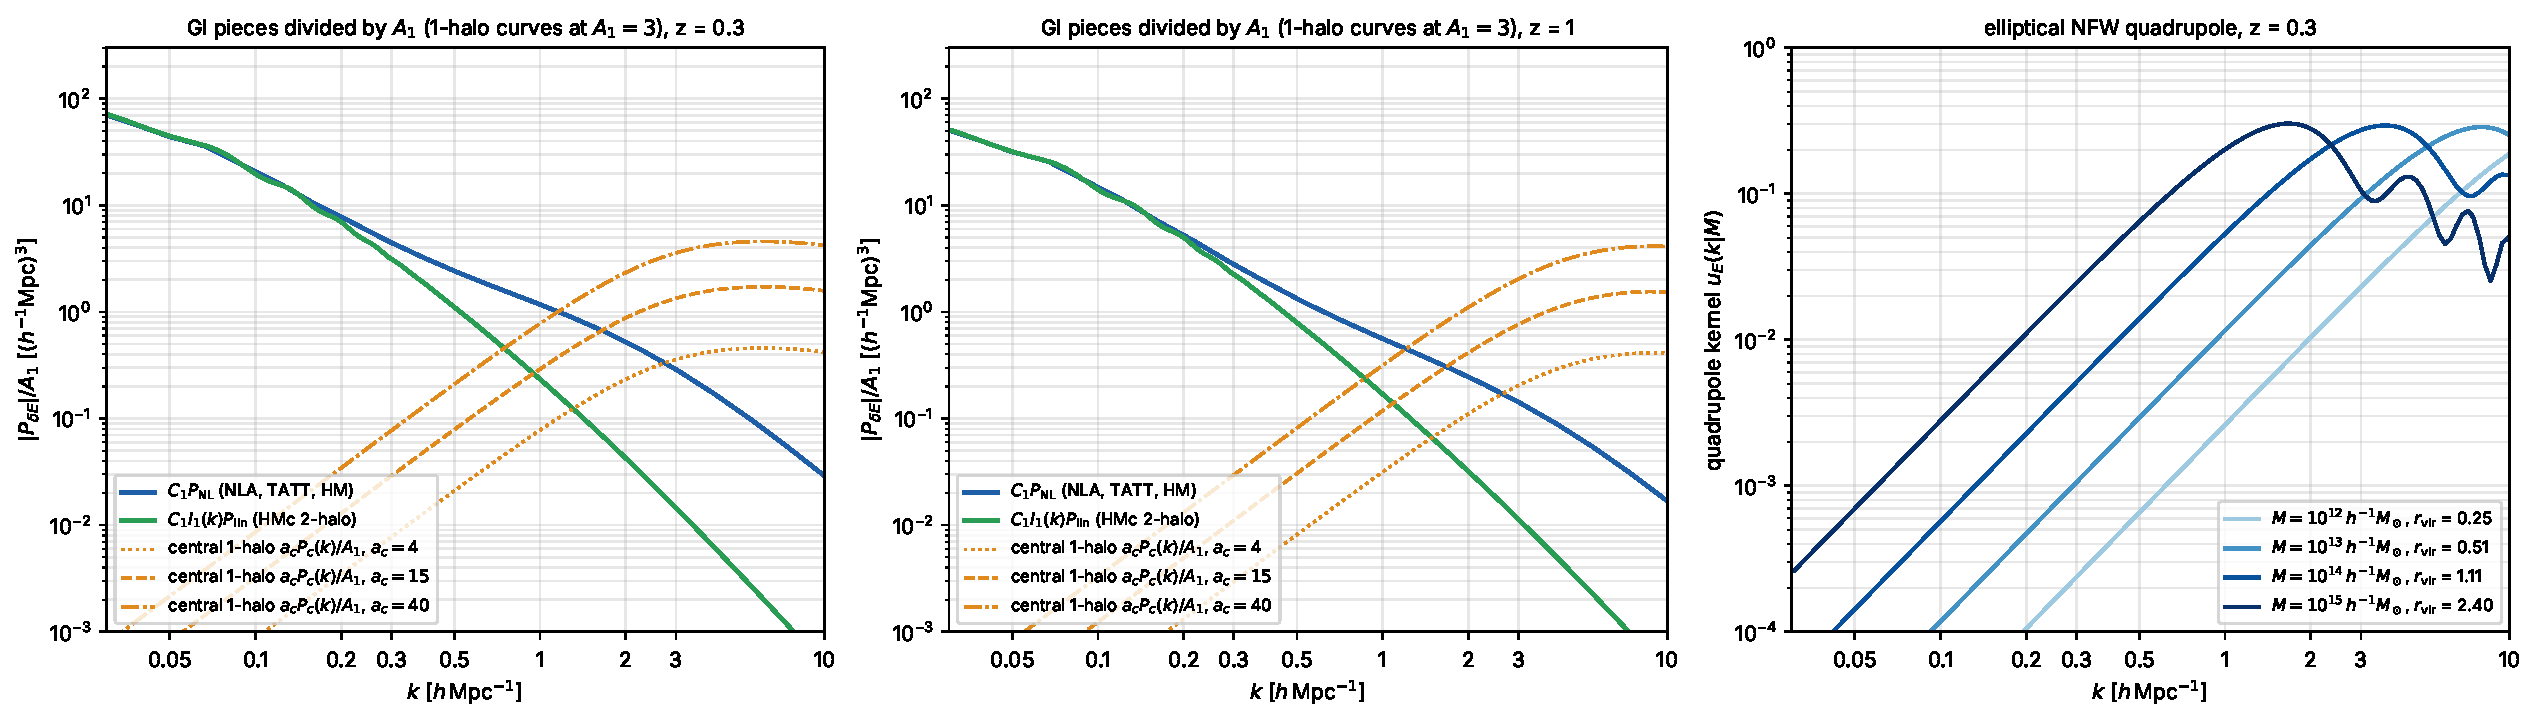
\includegraphics[width=\textwidth]{fig_hmc_terms}
\caption{Anatomy of the GI term. Left, middle: the centrals' GI per unit $A_1$
in NLA, TATT and HM ($\bar C_1\PNL$, blue) and in HMc: 2-halo
$\bar C_1 I_1\Plin$ (green) plus the central 1-halo term (orange, three $a_c$).
$\PNL$ adds the full own-halo matter at full alignment strength; HMc lets the
data set it. Right: the quadrupole kernel $u_E(k|M)$, Eq.~\eqref{eq:uE}.}
\label{fig:terms}
\end{figure}

\section{FLAMINGO tests}
Data: FLAMINGO shape spectra converted to the cosmolike convention, snapshots
$z = 0.2$ to 2; probes $P_{hE}$ ($\tfrac32\times$ monopole), $P_{EE}$, $P_{BB}$;
$0.05 \le k \le \kmax$; $N_s$ fixed to the $B$ plateau; FLAMINGO $\PNL$ and $b(k)$;
$\nu = 3N_k - n_{\rm par}$. Cut: last $\kmax$ before two consecutive $p < 0.05$.
(The FLAMINGO errors are underestimated by 3 to 9 times at high $k$, so absolute
$\chi^2/\nu$ at $\kmax \gtrsim 1$ is inflated; the comparisons between models stand.)

\begin{table}[H]\centering\footnotesize
\caption{Summed $\chi^2_{\min}/\nu$ over the nine snapshots against $\kmax$
[$h\,$Mpc$^{-1}$], and the goodness-of-fit cuts. ``$\beta$'', ``$p$'': $a_c \propto
(M/10^{13.5})^\beta$ and $\mathsf E(r) \propto (r/r_{\rm vir})^p$, profiled on grids
(both run to their grid edges and help only at $k \ge 2$).}
\label{tab:gof}
\resizebox{\textwidth}{!}{\begin{tabular}{l c cccccc l}\toprule
model & $n_{\rm par}$ & 0.29 & 0.39 & 0.52 & 0.94 & 1.69 & 3.04 & cuts ($z = 0.2 \ldots 2$)\\ \midrule
TATT & 3 & 1.45 & 2.88 & 8.32 & 62.89 & 53.39 & 60.44 & .22 .22 .22 .29 .29 .29 .29 .29 .39\\
HM (TATT on $P_{\rm NL}$ + F21 satellites) & 4 & 1.54 & 3.00 & 8.44 & 58.57 & 49.18 & 41.69 & .22 .22 .22 .29 .29 .29 .29 .29 .39\\
\addlinespace
HM + central 1h, $P_{\rm NL}$ kept & 5 & 1.35 & 1.71 & 2.78 & 17.01 & 32.05 & 43.94 & .22 .29 .29 .39 .39 .29 .39 .29 .39\\
HMc, II on $P_{\rm NL}$ & 5 & 2.09 & 3.82 & 6.85 & 20.55 & 18.47 & 28.70 & .22 .22 .16 .22 .16 .22 .22 .29 .39\\
\textbf{HMc} & 5 & 1.31 & 1.80 & 2.80 & 13.05 & 12.65 & 24.51 & .22 .29 .29 .39 .39 .39 .39 .29 .39\\
\addlinespace
HMc + $\beta$ (mass dependence) & 6 & 1.42 & 1.92 & 2.95 & 13.56 & 12.63 & 17.99 & .22 .29 .29 .29 .39 .39 .39 .29 .39\\
HMc + $p$ (radial profile) & 6 & 1.42 & 1.92 & 2.96 & 13.59 & 12.97 & 22.89 & .22 .29 .29 .29 .39 .39 .39 .29 .39\\
HMc + coherent satellites & 5 & 0.79 & 0.80 & 0.98 & 2.22 & 4.13 & 14.37 & .70 .70 .70 .52 .70 .70 .70 .70 .70\\
\addlinespace
TATT + $W$ & 4 & 1.04 & 1.78 & 5.73 & 20.92 & 20.88 & 48.47 & .29 .29 .29 .29 .29 .39 .39 .70 .70\\
\textbf{HMc + $W$} & 6 & 0.85 & 0.85 & 1.04 & 2.28 & 4.22 & 14.65 & .70 .70 .70 .52 .70 .52 .70 .70 .70\\
\addlinespace
TATT + $W$, constant $b_g$ (no measured $b(k)$) & 4 & 0.98 & 2.00 & 6.90 & 24.34 & 24.52 & 58.88 & .29 .29 .29 .29 .29 .39 .39 .70 .70\\
\textbf{HMc + $W$, halo-model $I_g(k)$ (no measured $b(k)$)} & 5 & 0.79 & 0.90 & 1.14 & 2.29 & 4.25 & 15.76 & .94 .70 .70 .52 1.26 .52 .70 .52 .52\\
\bottomrule\end{tabular}
}
\end{table}

\begin{figure}[H]\centering
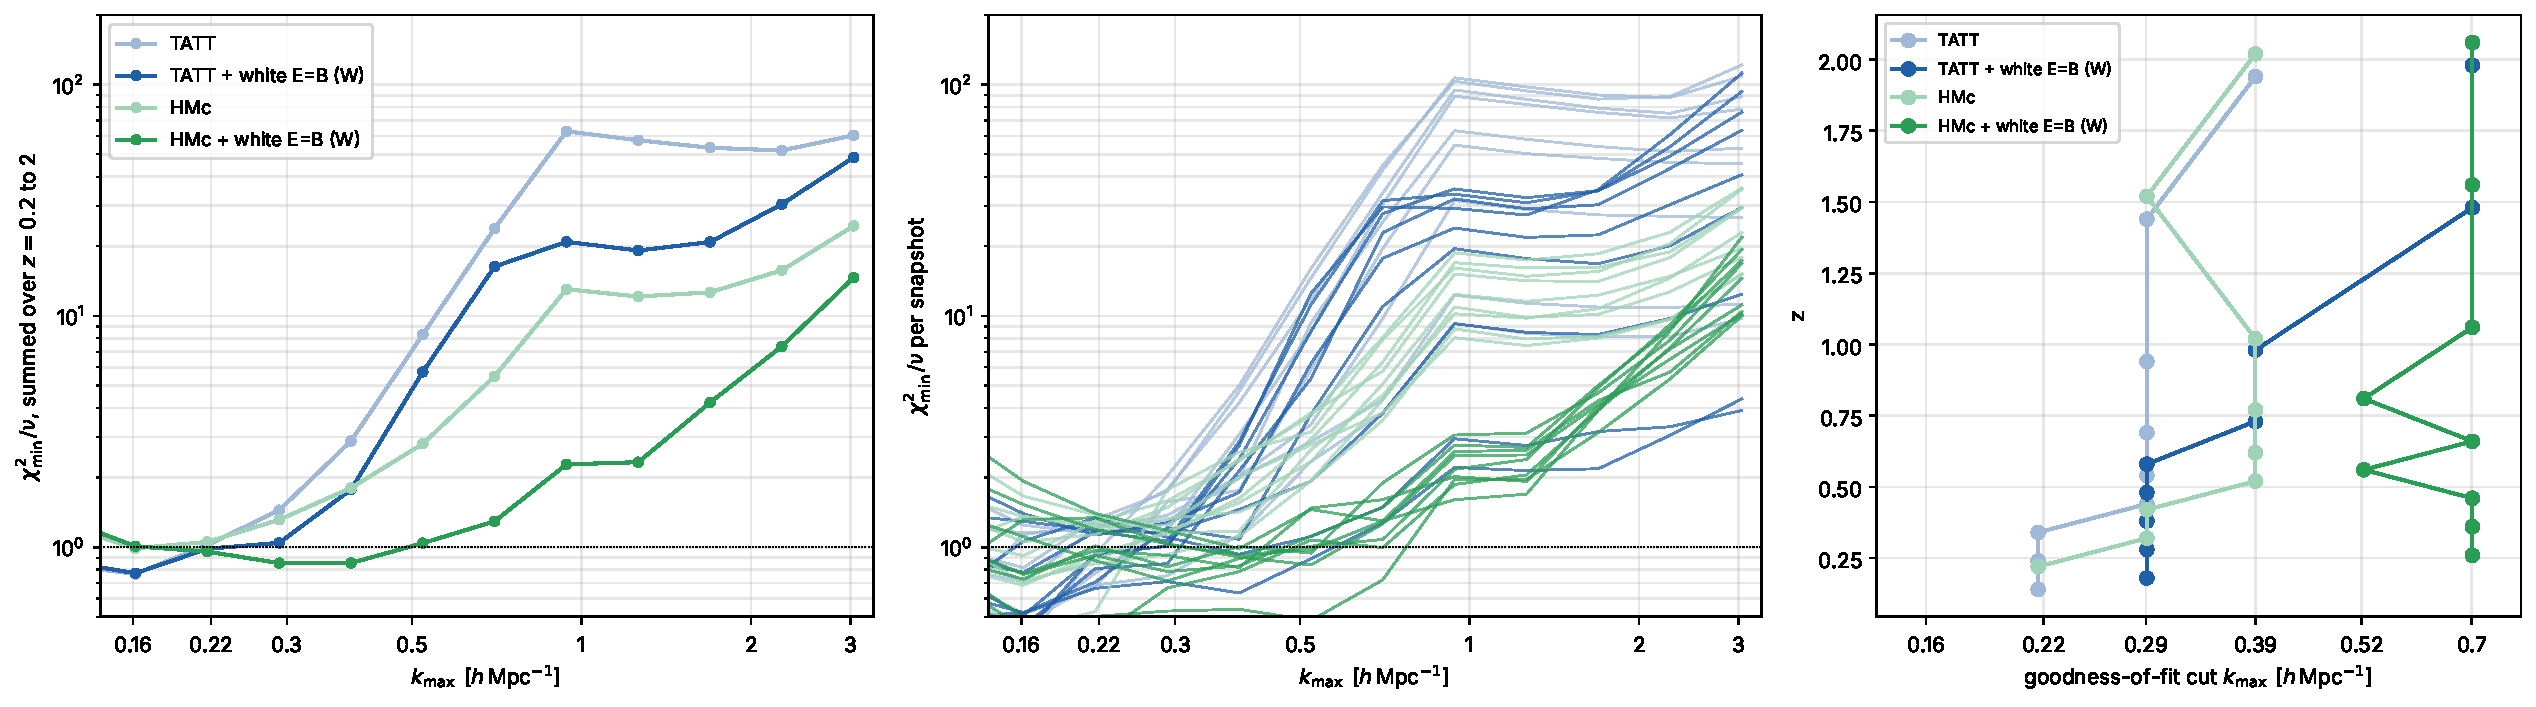
\includegraphics[width=\textwidth]{fig_hmcw_gof}
\caption{$\chi^2_{\min}/\nu$ against $\kmax$, summed (left) and per snapshot
(middle), and the goodness-of-fit cuts ($k$ horizontal, $z$ vertical; right).}
\end{figure}

\begin{figure}[H]\centering
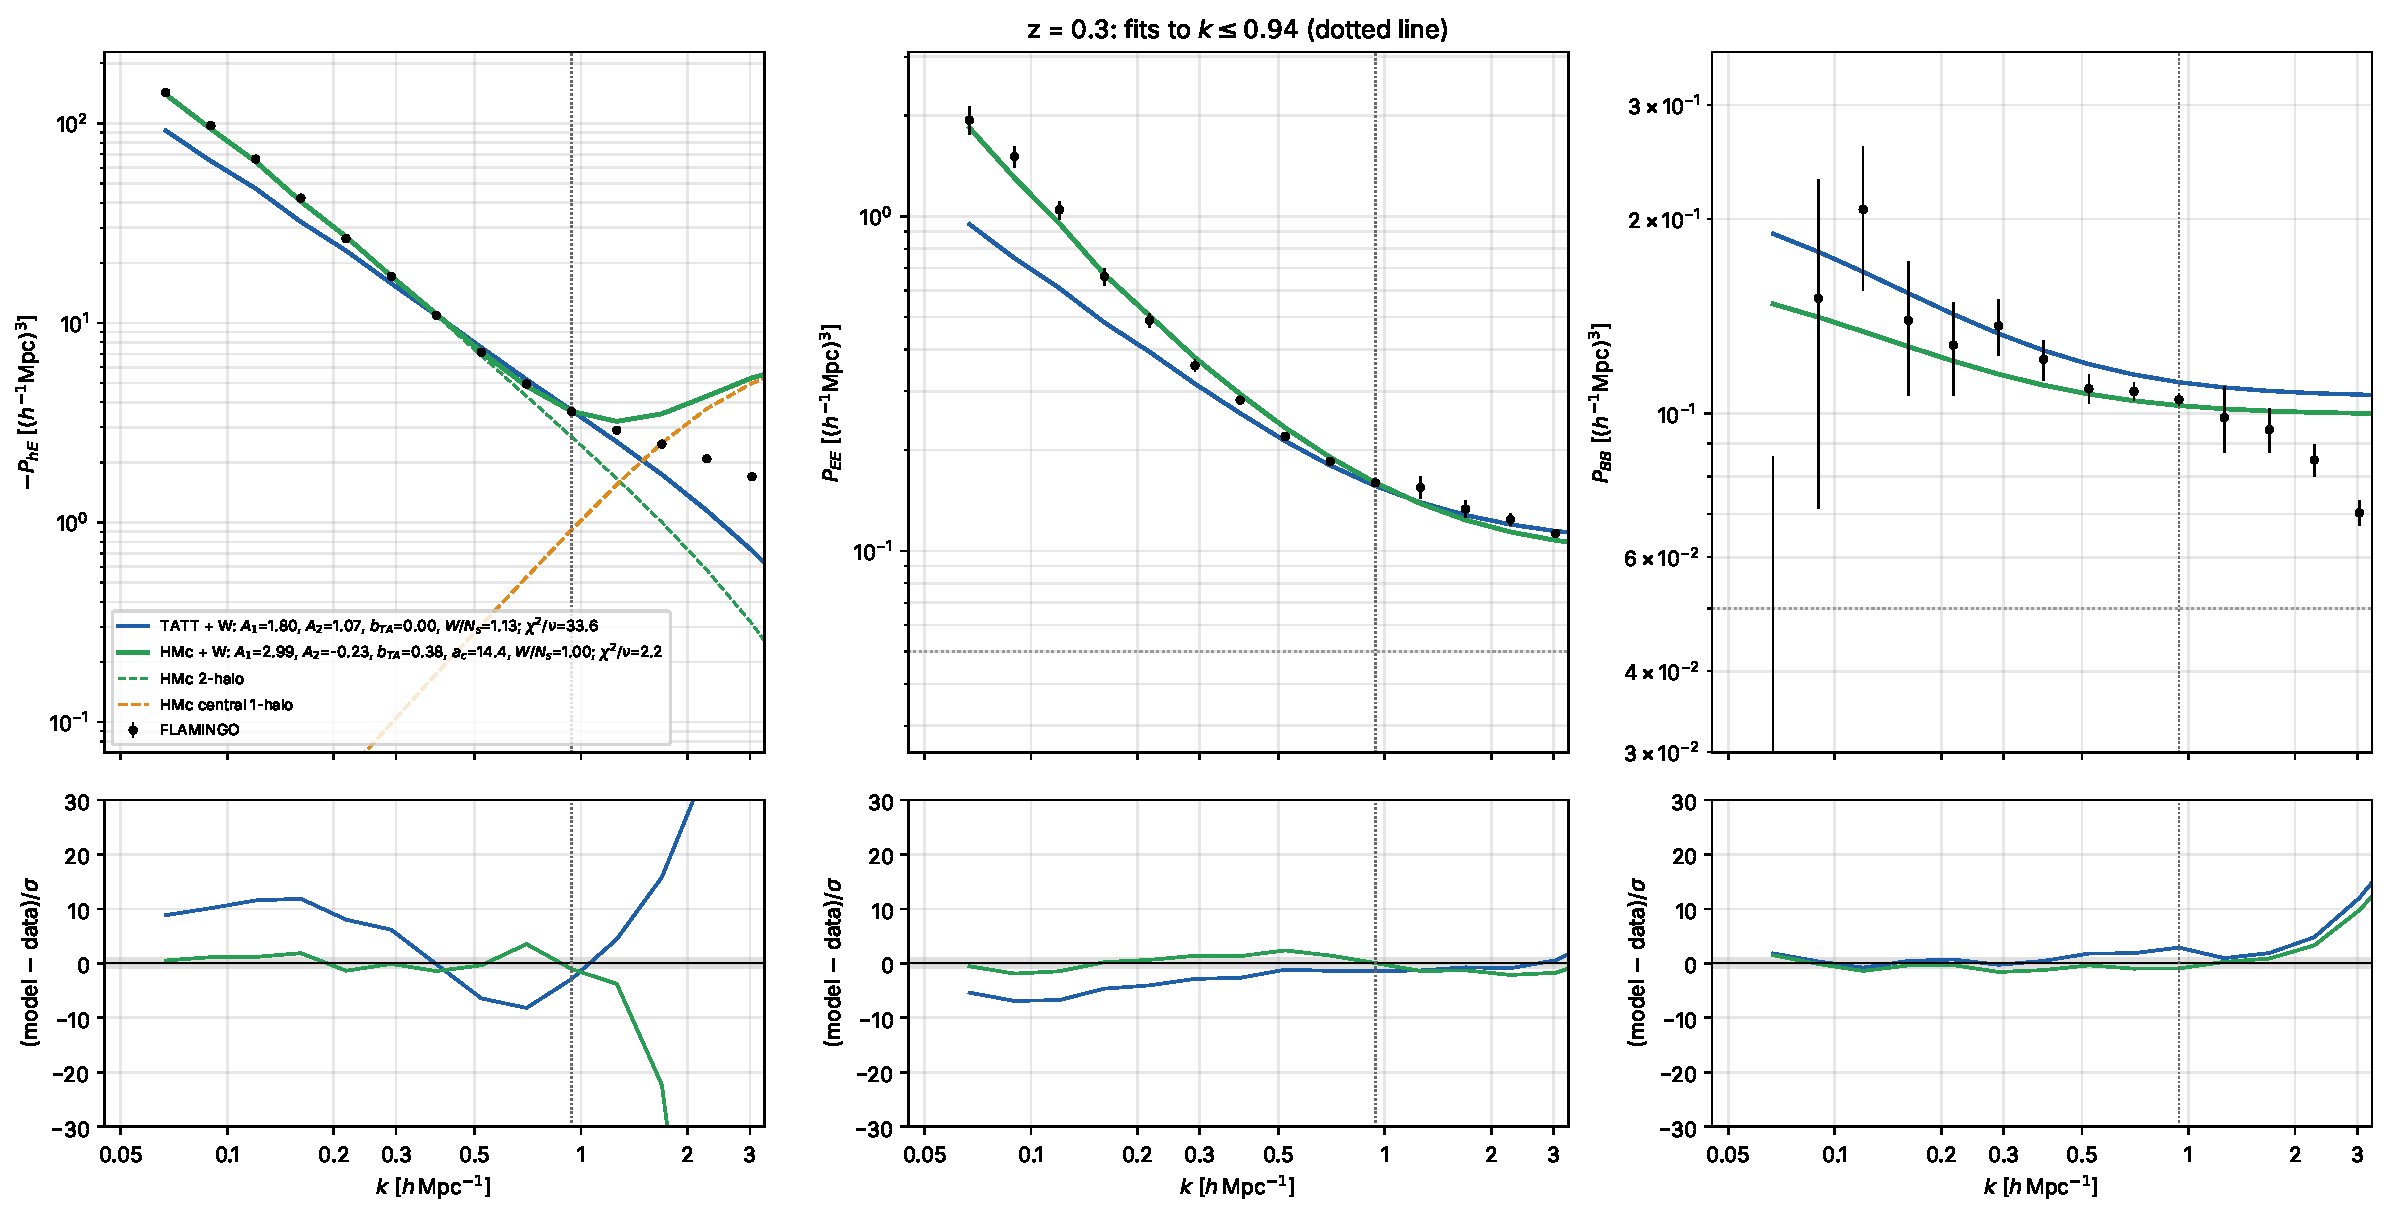
\includegraphics[width=\textwidth]{fig_hmcw_spectra_z0p3}
\caption{$z = 0.3$: TATT + $W$ (blue) and HMc + $W$ (green) fitted to
$k \le 0.94$; dashed: HMc 2-halo and central 1-halo GI. Bottom:
(model $-$ data)/$\sigma$. TATT must trade the low-$k$ GI amplitude against the
$k \sim 0.5$ excess; HMc fits $P_{hE}$ to $\lesssim 3\sigma$ up to the fit limit.}
\end{figure}

\begin{figure}[H]\centering
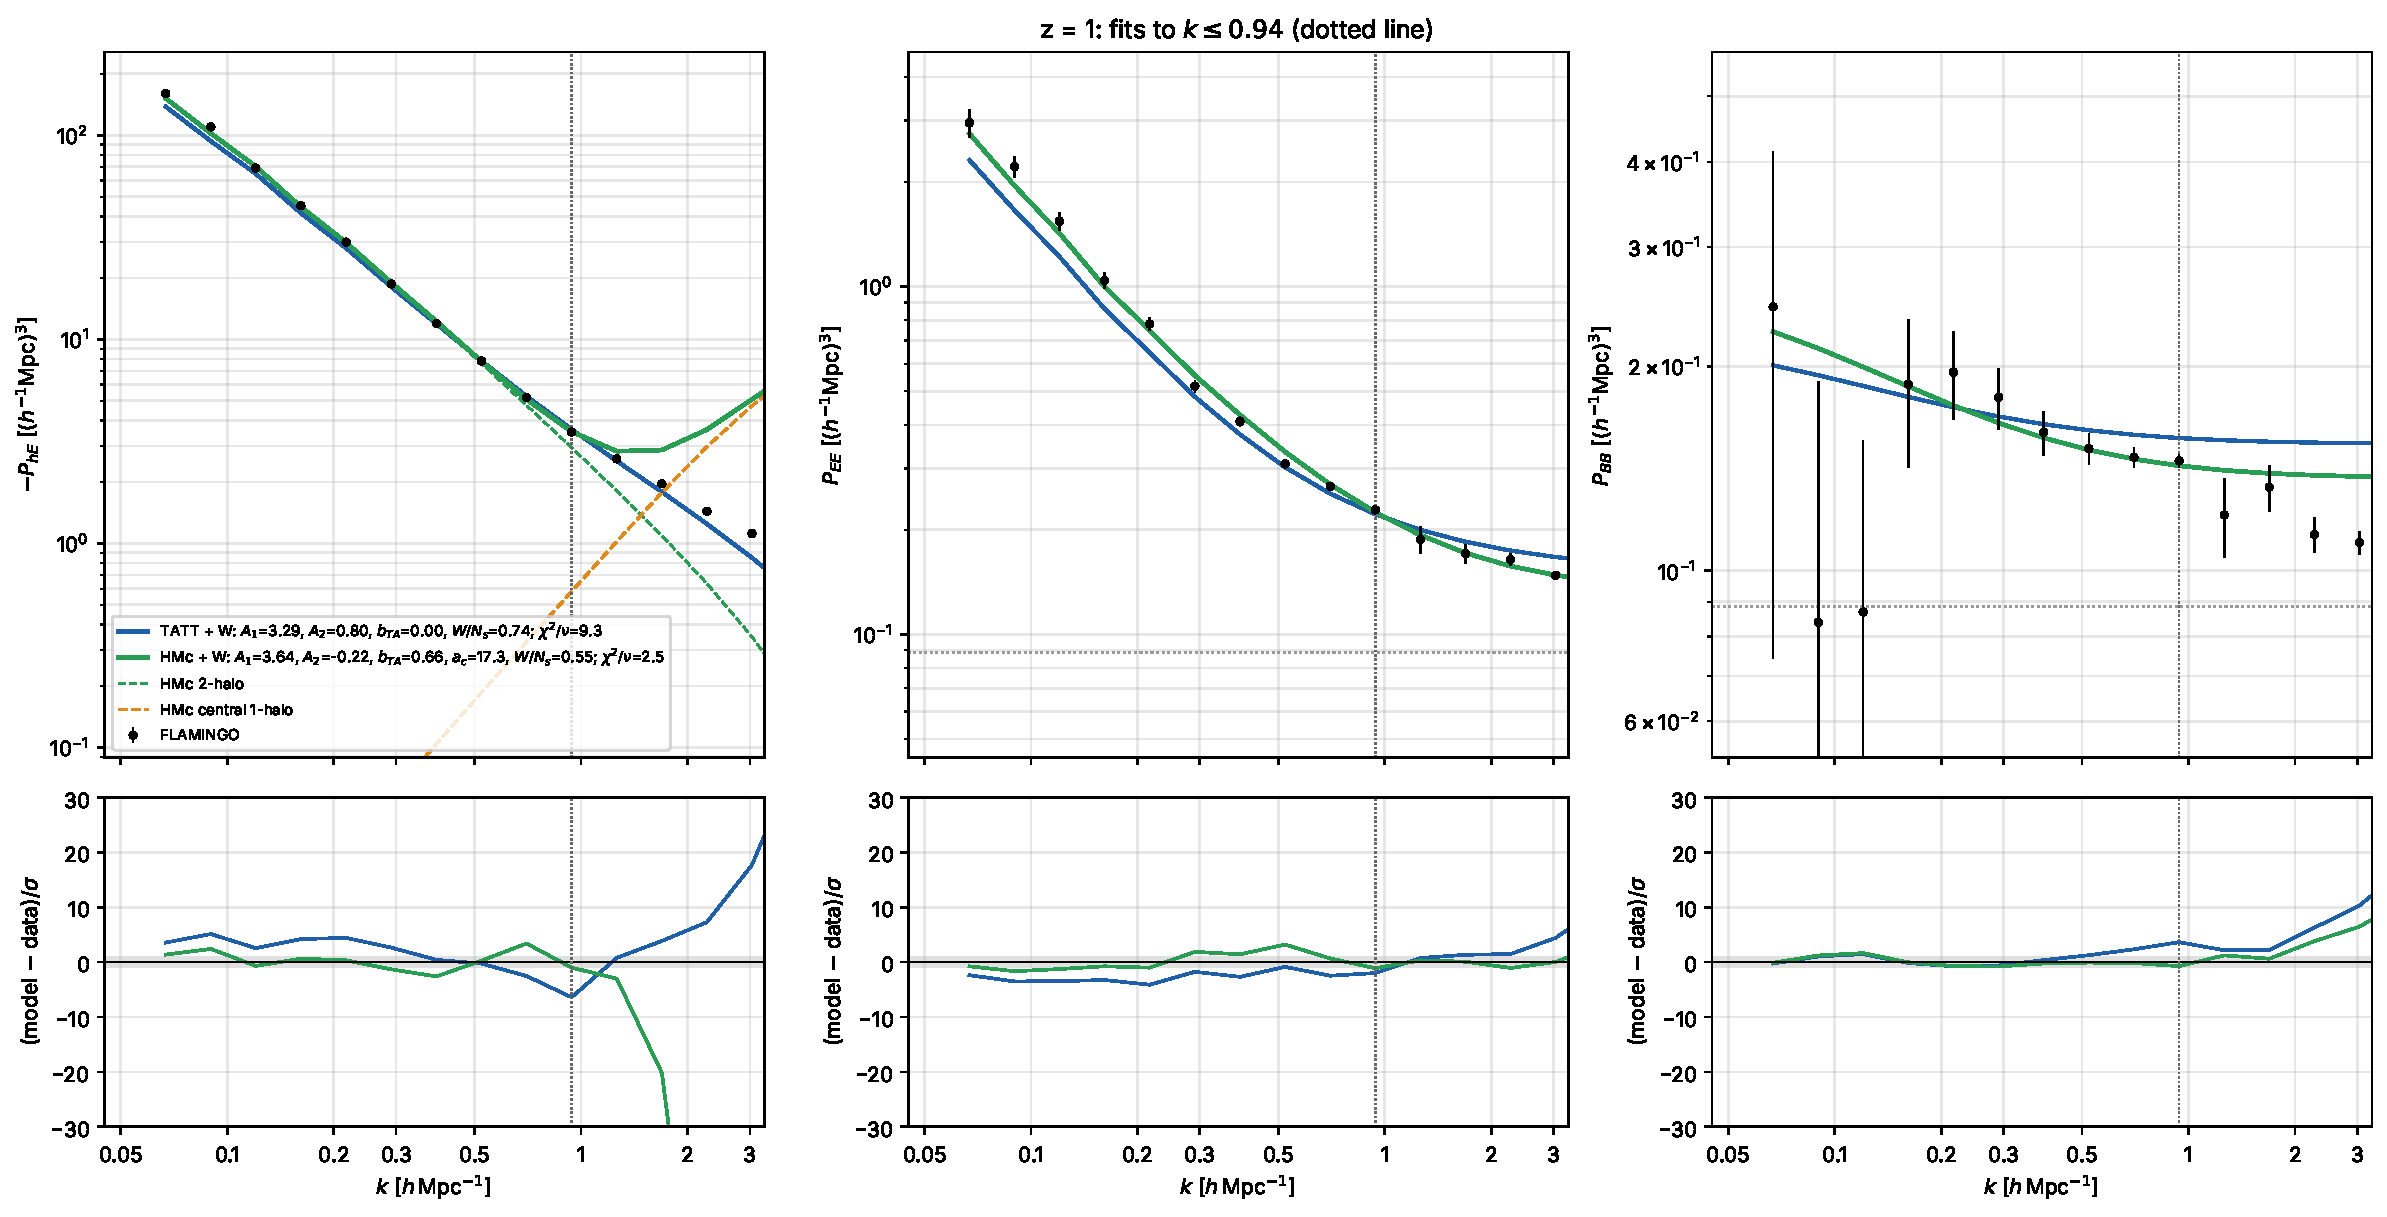
\includegraphics[width=\textwidth]{fig_hmcw_spectra_z1}
\caption{As above at $z = 1$.}
\end{figure}

\begin{table}[H]\centering\footnotesize
\caption{HMc + $W$ best-fit parameters per snapshot ($a_{1h} \simeq 0$ throughout).}
\resizebox{\textwidth}{!}{\begin{tabular}{c ccccccccccccccc}\toprule
 & \multicolumn{5}{c}{$k_{\max} = 0.52$} & \multicolumn{5}{c}{$k_{\max} = 0.94$} & \multicolumn{5}{c}{$k_{\max} = 3.04$}\\
\cmidrule(lr){2-6}\cmidrule(lr){7-11}\cmidrule(lr){12-16}
$z$ & $A_1$ & $A_2$ & $b_{\rm TA}$ & $a_c$ & $W/N_s$ & $A_1$ & $A_2$ & $b_{\rm TA}$ & $a_c$ & $W/N_s$ & $A_1$ & $A_2$ & $b_{\rm TA}$ & $a_c$ & $W/N_s$\\ \midrule
0.2 & 2.89 & -0.30 & 0.31 & 26.6 & 1.12 & 2.78 & -0.34 & 0.39 & 13.1 & 1.06 & 2.49 & -0.68 & 0.63 & 4.1 & 0.73\\
0.3 & 3.14 & -0.15 & 0.27 & 40.8 & 1.14 & 2.99 & -0.23 & 0.38 & 14.4 & 1.00 & 2.70 & -0.60 & 0.62 & 4.0 & 0.71\\
0.4 & 3.32 & -0.10 & 0.25 & 55.0 & 1.10 & 3.15 & -0.29 & 0.41 & 14.2 & 0.81 & 2.86 & -0.60 & 0.64 & 3.8 & 0.57\\
0.5 & 3.42 & -0.26 & 0.33 & 57.0 & 0.86 & 3.20 & -0.17 & 0.44 & 14.2 & 0.79 & 2.96 & -0.55 & 0.67 & 3.6 & 0.54\\
0.6 & 3.35 & -0.29 & 0.45 & 30.1 & 0.67 & 3.27 & -0.30 & 0.51 & 14.8 & 0.63 & 2.97 & -0.58 & 0.76 & 3.3 & 0.44\\
0.75 & 3.56 & -0.37 & 0.49 & 45.9 & 0.54 & 3.39 & -0.19 & 0.56 & 14.9 & 0.64 & 3.14 & -0.52 & 0.81 & 3.1 & 0.44\\
1 & 3.89 & -0.28 & 0.48 & 82.4 & 0.59 & 3.64 & -0.22 & 0.66 & 17.3 & 0.55 & 3.35 & -0.52 & 0.96 & 2.7 & 0.36\\
1.5 & 4.52 & -0.12 & 0.60 & 118.6 & 0.72 & 4.29 & -0.37 & 0.94 & 22.0 & 0.42 & 3.93 & -0.56 & 1.30 & 2.9 & 0.29\\
2 & 5.06 & 1.74 & 0.43 & 194.0 & 0.67 & 5.12 & -0.37 & 1.30 & 26.9 & 0.48 & 4.73 & -0.63 & 1.75 & 3.6 & 0.30\\
\bottomrule\end{tabular}
}
\end{table}

\paragraph{Reading.}
\begin{enumerate}[itemsep=2pt]
\item Keeping $\PNL$ and adding the central term on top fits only with
  $a_c \approx -85$ (anti-alignment): $\PNL$ already overcounts the own-halo
  GI. The consistent split (Eqs.~\ref{eq:gi2h}, \ref{eq:central}) is what works, and
  it needs the II on $\Plin$ too (``HMc, II on $\PNL$'' is worse).
\item With $W$ in both models, HMc beats TATT by a factor 5.5 in $\chi^2/\nu$ at
  $\kmax = 0.52$ and 9 at 0.94. At $\kmax = 0.52$ the remaining $\chi^2$ is then
  shared roughly evenly between $hE$, $EE$ and $BB$.
\item $a_c$ drifts with the fit range (27 to 190 at $\kmax = 0.52$, 13 to 27 at 0.94,
  3 to 4 at 3; the $\kmax = 0.52$ values grow with $z$, where the term is weakest): the central term rises as $k^2$ to $k \sim 3$ while FLAMINGO wants it to
  switch on earlier and level off. Neither a mass-dependent alignment nor a radial
  ellipticity profile fixes this at $k \le 1$; the likely cause is the halo model's
  known 2-halo deficit at $k \approx 0.3$ to 1, which a large $a_c$ compensates.
\item FLAMINGO's $BB$ excess over $N_s$ is white-like up to $k \sim 1$; a coherent
  satellite alignment reproduces it, but so does a constant.
\end{enumerate}

\section{Roman figure of bias}
Production pipeline (\texttt{v3/mask\_scan.py} masks, regenerated and checked
identical; \texttt{roman\_test.fit}): \texttt{example1\_cov}; data GG + FLAMINGO IA
through the sim-IA path; every parameter free; IA exact at the fiducial cosmology
and the cosmology response of the full model at the IA solution; case A
($\Omega_m$, $A_s$) and case B (+ $n_s$, $H_0$, $\Omega_b$ with the chain priors); FoB
uncertainty from the FLAMINGO errors. HMc is cosmolike's native TATT plus
per-snapshot templates through the same sim-IA path:
\begin{equation}
\xi_{\rm HMc} = \xi^{\rm native}_{\rm TATT} + \xi_{\rm sat}
 + \sum_s\Big[A_s\big(T^{GI,\rm lin}_s - T^{GI,\rm NL}_s\big) + A_s^2\big(T^{II,\rm lin}_s - T^{II,\rm NL}_s\big) + c_s T^{c}_s\Big],
\end{equation}
$A_s = A_1x_s^{\eta_1}$, $c_s = a_cx_s^{\eta_c}$, $x_s = (1+z_s)/1.62$; $T^{\rm lin}$: $A_1$
terms on $I_1\Plin$ (GI) and $\Plin$ (II); $T^{\rm NL}$: the same on $\PNL$; $T^c$:
Eq.~\eqref{eq:central}. Checks on the $K_0/D = 0.35$ mask: cosmolike's TATT $A_1$ term
equals its NLA exactly; the NLA templates reproduce native NLA to
$\Delta\chi^2 = 0.002$ (IA signal $\chi^2 = 1976$); the swap is worth
$\Delta\chi^2 = 0.8$ at $A_1 = 3.5$ and the central term $0.02$ at $a_c = 10$. The
templates are held at the fiducial cosmology.

\begin{figure}[H]\centering
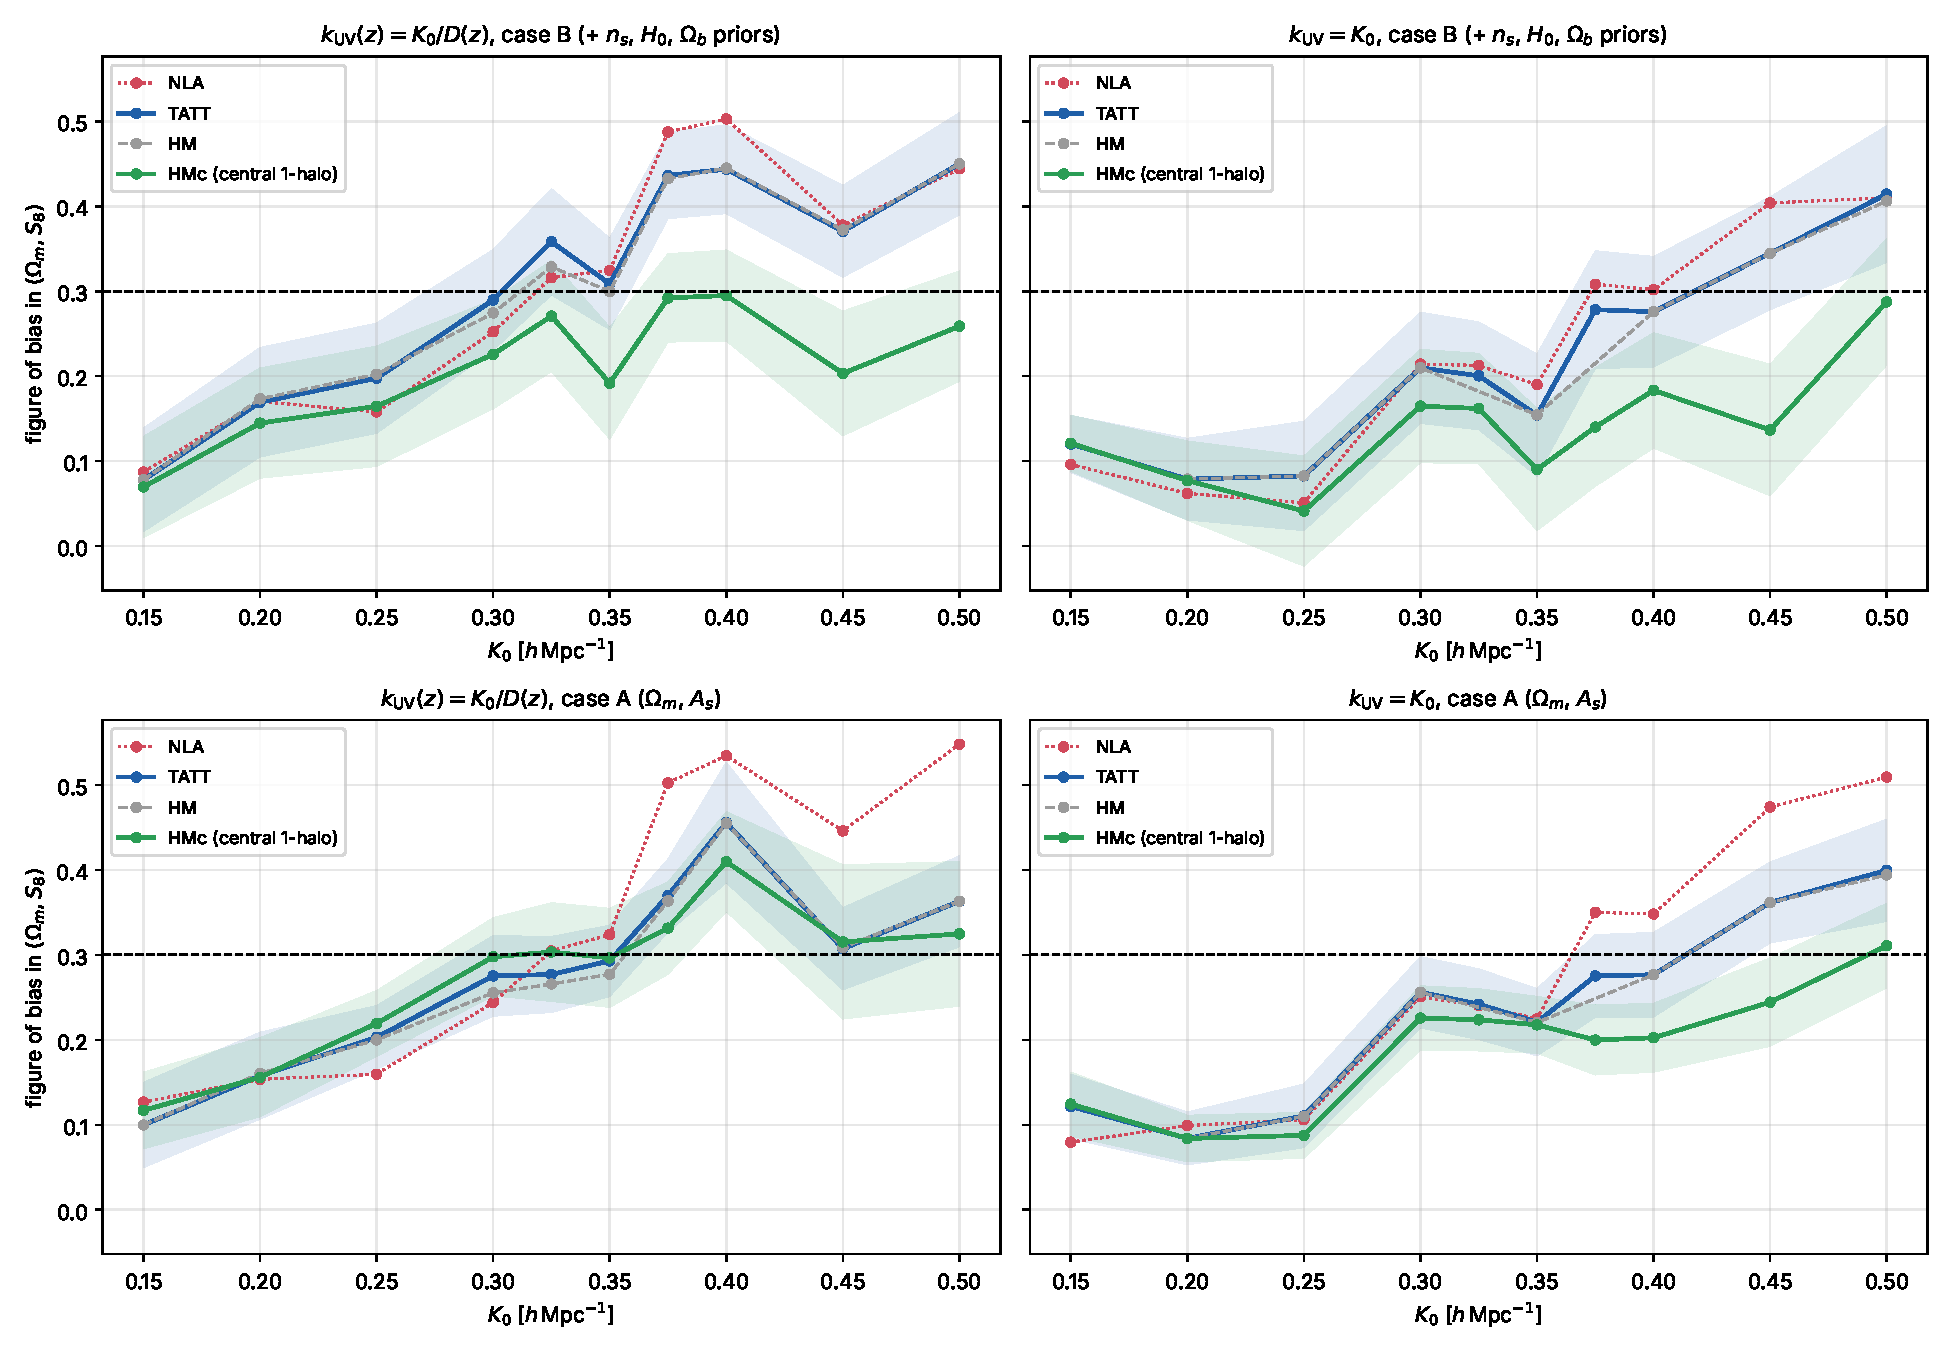
\includegraphics[width=\textwidth]{fig_hmc_fob}
\caption{FoB against $K_0$ for NLA, TATT, HM and HMc; bands: FoB uncertainty
from the FLAMINGO errors; dashed: 0.3.}
\end{figure}

\begin{table}[H]\centering\small
\caption{FoB, TATT and HMc (red: $> 0.3$).}
\begin{tabular}{c cc cc c cc cc}\toprule
 & \multicolumn{4}{c}{$k_{\rm UV}(z) = K_0/D(z)$} & & \multicolumn{4}{c}{$k_{\rm UV} = K_0$}\\
\cmidrule(lr){2-5}\cmidrule(lr){7-10}
 & \multicolumn{2}{c}{case B} & \multicolumn{2}{c}{case A} & & \multicolumn{2}{c}{case B} & \multicolumn{2}{c}{case A}\\
$K_0$ & TATT & HMc & TATT & HMc & & TATT & HMc & TATT & HMc\\ \midrule
0.15 & 0.08 & 0.07 & 0.10 & 0.12 &  & 0.12 & 0.12 & 0.12 & 0.12\\
0.2 & 0.17 & 0.14 & 0.16 & 0.16 &  & 0.08 & 0.08 & 0.08 & 0.08\\
0.25 & 0.20 & 0.16 & 0.20 & 0.22 &  & 0.08 & 0.04 & 0.11 & 0.09\\
0.3 & 0.29 & 0.23 & 0.28 & 0.30 &  & 0.21 & 0.16 & 0.26 & 0.23\\
0.325 & \textcolor{red!70!black}{0.36} & 0.27 & 0.28 & \textcolor{red!70!black}{0.30} &  & 0.20 & 0.16 & 0.24 & 0.22\\
0.35 & \textcolor{red!70!black}{0.31} & 0.19 & 0.29 & 0.30 &  & 0.15 & 0.09 & 0.22 & 0.22\\
0.375 & \textcolor{red!70!black}{0.44} & 0.29 & \textcolor{red!70!black}{0.37} & \textcolor{red!70!black}{0.33} &  & 0.28 & 0.14 & 0.28 & 0.20\\
0.4 & \textcolor{red!70!black}{0.44} & 0.29 & \textcolor{red!70!black}{0.46} & \textcolor{red!70!black}{0.41} &  & 0.28 & 0.18 & 0.28 & 0.20\\
0.45 & \textcolor{red!70!black}{0.37} & 0.20 & \textcolor{red!70!black}{0.31} & \textcolor{red!70!black}{0.32} &  & \textcolor{red!70!black}{0.34} & 0.14 & \textcolor{red!70!black}{0.36} & 0.24\\
0.5 & \textcolor{red!70!black}{0.45} & 0.26 & \textcolor{red!70!black}{0.36} & \textcolor{red!70!black}{0.32} &  & \textcolor{red!70!black}{0.41} & 0.29 & \textcolor{red!70!black}{0.40} & \textcolor{red!70!black}{0.31}\\
\bottomrule\end{tabular}

\end{table}

\paragraph{Reading.} Case B: HMc stays at or below 0.29 to $K_0 = 0.5$ in both
families (TATT: 0.36 at $K_0/D = 0.325$, 0.34 at constant 0.45). Case A: on $K_0/D$
both reach 0.3 near $K_0 = 0.3$ to 0.35; on constant $K_0$ HMc stays at or below
0.24 to 0.45 (TATT 0.36 there). HMc's best-fit $\chi^2$ is 0.1 to 0.45 above TATT's
on the $K_0/D$ masks and equal on the constant ones: HMc does not contain TATT, so
it is a different model with less bias, not a better fit to Roman. $a_c$ is
unconstrained on Roman's scales (often at 0, $\eta_c$ at its bounds).

\section{From one simulation cosmology to the whole prior}\label{sec:prior}
FLAMINGO exists at one cosmology, so it can test the model's \emph{form} there but
cannot supply anything the model needs elsewhere. The model is built so that it
does not have to:
\begin{center}\small
\begin{tabular}{p{4.2cm} p{5.4cm} p{6.0cm}}\toprule
ingredient & source & over the prior\\ \midrule
$\Plin$, $\PNL$, FAST-PT kernels & cosmolike & exact at every cosmology (now)\\
$I_1(k)$, $u_E(k|M)$, $P_c(k)$, satellite tables & halo model: Tinker mass function and bias, NFW, $c(M)$ & cosmology dependent; \textbf{currently held at the fiducial} (to fix)\\
halo shapes $\sigma_E^2(M)$ & Allgood et al.\ (2006), in $M/M_*$ & follows $M_*(z, \text{cosmology})$\\
HOD ($M_{\min}$, $M_1$) & sample property ($\bar n_g$, $b_g$) & held fixed in mass, or nuisance; enters only the weights $N_{c,s}/\bar n_g$\\
$A_1, A_2, \bTA, a_c, \eta$'s & free nuisance parameters & marginalised, as in TATT\\
$b(k)$ & FLAMINGO & not used by the model (Eq.~\ref{eq:nob})\\
\bottomrule\end{tabular}
\end{center}
The one real gap is the second row: on Roman the halo-model pieces are templates
at the fiducial cosmology, so at other cosmologies the $A_1$ term responds as
$\PNL$ and the central term not at all. The fix is to evaluate them at each
cosmology, most naturally in cosmolike's \texttt{halo.c}, which already has the
mass function, bias, NFW profiles and HOD for the F21 model: $I_1(k)$ is one more
integral, and $u_E$ is Eq.~\eqref{eq:uE}.

\section{Caveats and next steps}
\begin{itemize}[itemsep=2pt]
\item Evaluate $I_1$, $P_c$ and the satellite tables at each cosmology (cosmolike
  \texttt{halo.c}), and check the size of the fixed-template error on Roman.
\item Isolate the source of the Roman gain: rerun with $a_c = 0$ (swap only).
\item Fix the 1-halo/2-halo transition (free HMcode-style smoothing, or a
  CHEFT-type 2-halo with mass-dependent operators), which should remove the $a_c$
  drift.
\item Interpret $a_c$: needs the normalisation of FLAMINGO's shape estimator
  ($A_1 \approx 3$ to 4 here); cross-check halo shapes and central-halo misalignment
  in FLAMINGO itself (outside the fit, to avoid circularity).
\end{itemize}

\section{Addendum, 17 November 2026: the 1-halo amplitudes are not physical}\label{sec:addendum}
\newcommand{\figdir}{../../../notes/flamingo_vs_tng300/plots}

\paragraph{The problem.} With $\gamma^c_{ij} = a_c[\mathsf E_{ij}]_\perp$ and
$E_{ii} = 2\ln a_i$, a central with the axis ratios of its halo and perfectly
aligned with it has shear $\tfrac12\ln(a_1/a_2)$ to first order, which is
$a_c = 0.5$ (an estimate; misalignment lowers it). The HMc + $W$ fits give
$a_c = 27$ to 190 at $\kmax = 0.52$ and 13 to 27 at 0.94. At $z = 1$ the value
follows the fit range: 300 (the prior bound), 102, 82, 38, 17 and 2.7 for
$\kmax = 0.29$, 0.39, 0.52, 0.70, 0.94 and 3.04. A good $\chi^2$ with an
amplitude of this size is a failed fit; only the goodness of fit had been
checked.

\paragraph{The cause.} $I_1 \simeq 1$ below $k = 1$, so the swap of
Eq.~\eqref{eq:gi2h} is in effect $\PNL \to \Plin$: at $z = 1$ it removes 29, 42
and 56\% of the $A_1$ GI term at $k = 0.39$, 0.52 and 0.70$\hmpc$. The model
hands all of that power to the central 1-halo term, but a single halo's
quadrupole is suppressed as $(kr)^2$ below $k \sim 1/r_{\rm vir}$
(Eq.~\ref{eq:uE}). At $z = 1$, FLAMINGO minus the fitted 2-halo term is nearly
flat, 0.3 to 0.6$\,(h^{-1}{\rm Mpc})^3$ from $k = 0.5$ to 4$\hmpc$, while $P_c$
rises by a factor 30 over that range: the amplitude that one bin alone needs
falls from 49 at $k = 0.52$ to 1.8 at $k = 4.1$. No single $a_c$ fits, and the
fit to $\kmax = 0.70$ overshoots $P_{\delta E}$ by 51\% at $k = 1.3$ and 151\% at
1.7 (Fig.~\ref{fig:addold}).

\begin{figure}[H]\centering
\includegraphics[width=0.68\textwidth]{\figdir/ia_hmc_z1/ia_hmc_z1}
\caption{FLAMINGO at $z = 1$ (shear units, $\mu = 0$; $P_{\delta E} =
P_{hE}/b(k)$) and the HMc + $W$ fit with $a_c$ free, with its parts. Bottom
row: $100\,(\text{model} - \text{FLAMINGO})/\text{FLAMINGO}$, gray band: the
measurement error. Solid, filled: inside the fit range; dashed, open:
outside.}
\label{fig:addold}
\end{figure}

\paragraph{The test.} The $A_1$ terms were put on
\begin{equation}
P_{\rm GI} = I_1\Plin + \alpha\,(\PNL - I_1\Plin),\qquad
P_{\rm II} = \Plin + \alpha\,(\PNL - \Plin),
\end{equation}
with $\alpha$ free in $[-1, 2]$ (its physical range is 0 to 1; the wider range
lets an unphysical value show) and $a_c \le 1$; everything else as HMc + $W$.
Summed $\chi^2_{\min}/\nu$ over the nine snapshots:
\begin{center}\small
\begin{tabular}{lccc}\toprule
$\kmax$ [$h\,$Mpc$^{-1}$] & 0.52 & 0.70 & 0.94\\ \midrule
HMc + $W$ ($a_c \le 300$) & 1.04 & 1.29 & 2.28\\
HMc + $W$, $a_c \le 1$ & 2.17 & 4.49 & 8.73\\
$\alpha$ free, $a_c \le 1$ & 1.03 & 1.11 & 1.18\\
$\alpha$ free, $a_c \le 1$, no satellites ($a_{1h} = 0$) & 0.97 & 1.08 & 1.33\\
\bottomrule\end{tabular}
\end{center}
HMc cannot fit with a physical $a_c$ (second row); with $\alpha$ it fits
better than with $a_c$ free, at the same number of parameters when the
satellites are off.

\paragraph{Physical-sensibility checks of the refit} (no satellites unless
stated; \texttt{hmc\_alpha\_checks.py}).
\begin{itemize}[itemsep=1pt]
\item \emph{Passed.} $\alpha$ lies between 0.31 and 0.83 at every snapshot for
  $\kmax = 0.52$ to 0.94. At $z = 1$ ($\kmax = 0.70$): $\alpha = 0.58 \pm 0.06$,
  $A_1 = 4.03 \pm 0.07$ (the low-$k$ NLA value is 3.98); for $\kmax = 0.52$ to
  1.26, $A_1$ stays at 4.03 to 4.04 and $\alpha$ at 0.56 to 0.59. All spectra
  are positive. Outside the fit range the model degrades smoothly: $-6.5\%$ at
  $k = 1.3$ and $-13.5\%$ at 1.7 (Fig.~\ref{fig:add}, top). The
  goodness-of-fit cuts are 0.70 to 1.69$\hmpc$, against 0.52 to 0.70.
\item \emph{Failed: $a_c$ is unconstrained.} It sits at 0 or at the bound 1 in
  nearly every fit; at $a_c = 1$ the central term is below 2\% of
  $P_{\delta E}$ up to $k = 1.3$. FLAMINGO does not test the central 1-halo
  term at a physical amplitude.
\item \emph{Failed: the satellite amplitude.} With $a_{1h}$ free it is
  unconstrained for $\kmax \lesssim 1$ ($1.0 \pm 600$ at $z = 1$,
  $\kmax = 0.70$) and that value drives the model above the fit range. Where
  it is constrained it follows the fit range like $a_c$ did: 0.07, 0.04, 0.02
  and 0.009 for $\kmax = 1.26$, 1.69, 2.27 and 3.04 at $z \le 0.5$. At $z = 1$,
  $\kmax = 1.69$: $a_{1h} = 0.10 \pm 0.03$, which reaches the cap of 0.3 inside
  $0.58\,r_{\rm vir}$, and the model overshoots $P_{\delta E}$ by 28\% at
  $k = 2.3$ and 100\% at 3.0 (Fig.~\ref{fig:add}, bottom).
\item \emph{Limits of $\alpha$.} It is anticorrelated with $\bTA$ (correlation
  $-0.8$ to $-0.9$), rises with redshift (at $\kmax = 0.70$: 0.38 to 0.46 for
  $z \le 0.75$, 0.58 at $z = 1$, 0.78 at $z \ge 1.5$) and with $\kmax$ above 1.
  It is a phenomenological share, not a derived quantity. Without satellites
  the model underpredicts $P_{\delta E}$ by 7 to 20\% above $k = 1.2$.
\end{itemize}

\paragraph{What changes in this review.} Item 3 of the Reading of the FLAMINGO
tests (the drift of $a_c$) is the main result, not a detail: the central term
absorbed the 2-halo deficit. Neither 1-halo term of the model has the scale
dependence FLAMINGO needs; both rise too steeply with $k$. The 2-halo part
with $\alpha$ is the piece that passes the checks. The Roman scan was not
rerun with $\alpha$; there $a_c$ is unconstrained and the gain was already
attributed to the swap, which $\alpha \approx 0.5$ says goes too far by about
half.

\begin{figure}[H]\centering
\includegraphics[width=0.66\textwidth]{\figdir/ia_hmca_z1/ia_hmca_z1}\\[2pt]
\includegraphics[width=0.66\textwidth]{\figdir/ia_hmcas_z1/ia_hmcas_z1}
\caption{As Fig.~\ref{fig:addold} for the refit. Top: $\alpha$ free,
$a_c \le 1$, no satellites. Bottom: the same with the satellites free, fitted
to a wider range. The central 1-halo term has no $P_{EE}$ part: one central
per halo.}
\label{fig:add}
\end{figure}

\section*{Code}
Addendum: \texttt{notes/flamingo\_vs\_tng300/fits/hmc\_alpha\_fit.py} (the refit,
\texttt{hmc\_alpha\_fits.json}), \texttt{hmc\_alpha\_checks.py} (the checks,
\texttt{checks\_z1.txt}), \texttt{notes/flamingo\_vs\_tng300/plots/} (figures).

\texttt{v6/halo\_central.py} (central tables), \texttt{halo\_central\_grid.py}
($\beta$, $p$ grids), \texttt{halo\_satcoh.py} (coherent satellites),
\texttt{halo\_central\_fit.py} (FLAMINGO fits, \texttt{f21v\_<variant>.npz}),
\texttt{hmc\_scan.py} (Roman scan, \texttt{hmc\_scan\_ex1\_\{D1,flat\}.json}),
\texttt{make\_hmcw.py}, \texttt{make\_hmc\_roman.py}, \texttt{make\_hmc\_review.py}
(figures, tables).
\end{document}
